\documentclass[titlepage]{article}
\usepackage[utf8]{inputenc}
\usepackage{amsmath}
\usepackage{amssymb}
\usepackage{booktabs}
\usepackage{algorithm}
\usepackage{algpseudocode}
\usepackage{pdfpages}
\usepackage{graphicx} % Necessario per \includegraphics
\usepackage{float}    % Aggiunto per forzare la posizione con [H]

\title{Second Assignment: Dataflow analysis}
\author{Carmine De Rosa \\ Manuel Gherardi \\ Arild Kuti}
\date{}
\begin{document}
\maketitle

% ==========================================
% SECTION 1: VERY BUSY EXPRESSIONS
% ==========================================
\section{Very Busy Expressions}

An expression is defined as a \textit{very busy expression} at a point \textit{p} if any path starting from \textit{p} uses the expression without redefining any of its operands. \\
To identify them, we proceed backward, starting from the \textit{Exit} basic block of the Control Flow Graph (CFG), applying the transfer function and using the intersection ($\cap$) as the meet operator.

\begin{table}[H] % Cambiato in [H]
\centering
\renewcommand{\arraystretch}{1.5}
\begin{tabular}{ll}
\toprule
\textbf{Parameter} & \textbf{Definition} \\
\midrule
\textbf{Domain} & Sets of expressions \\
\textbf{Direction} & Backward: $in[b] = f_b(out[b])$, $out[b] = \wedge in[succ(b)]$ \\
\textbf{Transfer Function} & $in[b] = Gen_b \cup (out[b] \setminus Kill_b)$ \\
\textbf{Meet Operation ($\wedge$)} & Intersection ($\cap$) \\
\textbf{Boundary Condition} & $in[\text{Exit}] = \emptyset$ \\
\textbf{Initial Interior Points} & $in[B] = S$ (Universal set) \\
\bottomrule
\end{tabular}
\caption{Very Busy Expressions parameters}
\end{table}

\begin{algorithm}[H] % Cambiato in [H]
\caption{Very Busy Expressions Algorithm}
\begin{algorithmic}[1]
\State $in[\text{Exit}] \gets \emptyset$
\For{\textbf{each} basic block $B \neq \text{Exit}$}
    \State $in[B] \gets S$
\EndFor
\Statex
\State $changes \gets \text{true}$
\While{$changes$}
    \State $changes \gets \text{false}$
    \For{\textbf{each} basic block $B \neq \text{Exit}$}
        \State $out[B] \gets \bigcap_{a \in succ(B)} in[a]$
        \State $in_{new} \gets Gen_B \cup (out[B] \setminus Kill_B)$
        \If{$in[B] \neq in_{new}$}
            \State $in[B] \gets in_{new}$
            \State $changes \gets \text{true}$
        \EndIf
    \EndFor
\EndWhile
\end{algorithmic}
\end{algorithm}

\begin{figure}[H] % Aggiunto [H] qui per bloccare l'immagine
    \centering
    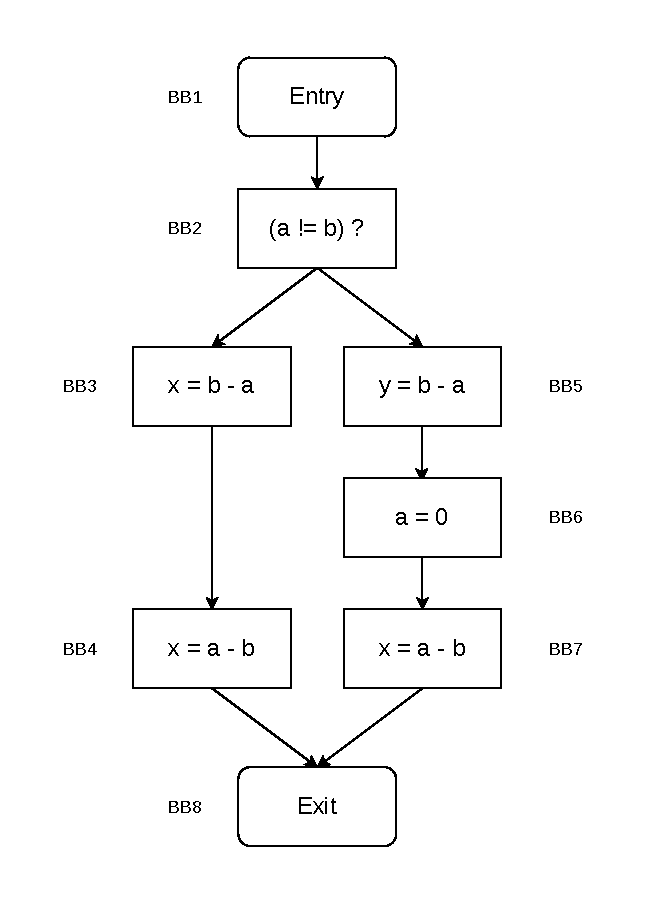
\includegraphics[width=1.0\linewidth]{very_busy_expressions.pdf}
    \caption{Very busy expression example CFG}
\end{figure}

\vspace{0.5cm}

\begin{table}[H] % Cambiato in [H]
\centering
\renewcommand{\arraystretch}{1.5}
\begin{tabular}{lcccccc}
\toprule
 & \multicolumn{2}{c}{\textbf{Iteration 1}} & \multicolumn{2}{c}{\textbf{Iteration 2}} & \multicolumn{2}{c}{\textbf{Iteration 3}} \\
\cmidrule(lr){2-3} \cmidrule(lr){4-5} \cmidrule(lr){6-7}
\textbf{Basic Block} & \textbf{IN[B]} & \textbf{OUT[B]} & \textbf{IN[B]} & \textbf{OUT[B]} & \textbf{IN[B]} & \textbf{OUT[B]} \\
\midrule
\textbf{BB1} & $\langle \dots \rangle$ & $\langle \dots \rangle$ & & & & \\
\textbf{BB2} & & & & & & \\
\textbf{BB3} & & & & & & \\
\textbf{BB4} & & & & & & \\
\textbf{BB5} & & & & & & \\
\textbf{BB6} & & & & & & \\
\textbf{BB7} & & & & & & \\
\textbf{BB8} & & & & & & \\
\bottomrule
\end{tabular}
\caption{Iteration table for example CFG}
\end{table}

\clearpage
\clearpage % Manda le prossime sezioni su una nuova pagina

% ==========================================
% SECTION 2: DOMINATOR ANALYSIS
% ==========================================
\section{Dominator Analysis}

L'analisi dei Dominatori è fondamentale per la costruzione della Static Single Assignment (SSA) form e per l'individuazione dei loop naturali nel Control Flow Graph. Un nodo $d$ domina un nodo $n$ se ogni percorso dal nodo di ingresso al nodo $n$ deve passare per $d$.

\begin{table}[H] % Cambiato in [H]
\centering
\renewcommand{\arraystretch}{1.5}
\begin{tabular}{ll}
\toprule
\textbf{Parameter} & \textbf{Definition} \\
\midrule
\textbf{Domain} & Sets of expressions \\
\textbf{Direction} & Backward: $in[b] = f_b(out[b])$, $out[b] = \wedge in[succ(b)]$ \\
\textbf{Transfer Function} & $in[b] = Gen_b \cup (out[b] \setminus Kill_b)$ \\
\textbf{Meet Operation ($\wedge$)} & Intersection ($\cap$) \\
\textbf{Boundary Condition} & $in[\text{Exit}] = \emptyset$ \\
\textbf{Initial Interior Points} & $in[B] = S$ (Universal set) \\
\bottomrule
\end{tabular}
\caption{Dominator Analysis parameters}
\end{table}

\begin{algorithm}[h!]
\caption{Calcolo dei Dominatori (TBD)}
\begin{algorithmic}[1]
\State \Comment{Algoritmo da definire...}
\end{algorithmic}
\end{algorithm}

\vspace{1cm}

% ==========================================
% SECTION 3: CONSTANT PROPAGATION
% ==========================================
\section{Constant Propagation}

La Constant Propagation è un'analisi dataflow progettata per determinare quali variabili all'interno di un programma hanno un valore costante in un determinato punto dell'esecuzione, permettendo al compilatore di sostituire la variabile con la costante stessa.

\begin{table}[H] % Cambiato in [H]
\centering
\renewcommand{\arraystretch}{1.5}
\begin{tabular}{ll}
\toprule
\textbf{Parameter} & \textbf{Definition} \\
\midrule
\textbf{Domain} & Sets of expressions \\
\textbf{Direction} & Backward: $in[b] = f_b(out[b])$, $out[b] = \wedge in[succ(b)]$ \\
\textbf{Transfer Function} & $in[b] = Gen_b \cup (out[b] \setminus Kill_b)$ \\
\textbf{Meet Operation ($\wedge$)} & Intersection ($\cap$) \\
\textbf{Boundary Condition} & $in[\text{Exit}] = \emptyset$ \\
\textbf{Initial Interior Points} & $in[B] = S$ (Universal set) \\
\bottomrule
\end{tabular}
\caption{Contant Propagation parameters}
\end{table}

\begin{algorithm}[h!]
\caption{Constant Propagation (TBD)}
\begin{algorithmic}[1]
\State \Comment{Algoritmo da definire...}
\end{algorithmic}
\end{algorithm}

\end{document}